%WRITTEN BY: Daniel
\subsection{Deployment}

\subsubsection{Architecture}\hfill\\
Every configuration management tool requires an architecture which supports the management of a set of hosts. Chef and Puppet both implement a Master-Agent design where there exists a centralized control server and an agent program is installed on every managed device [Fig. \ref{fig:architecture}]. The centralized control server is responsible to keep a canonical state of configuration as provided by the operator in a repository and translates the configuration into profiles for every node.


\begin{figure*}
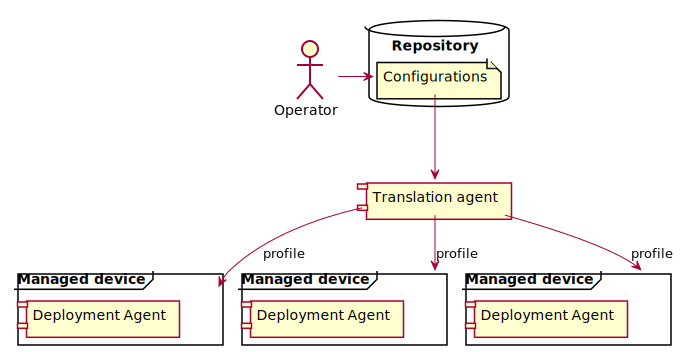
\includegraphics[height=2in]{assets/architecture}
\caption{Architecture of a centralized configuration management tool \cite{delaet2010survey}}
\label{fig:architecture}
\end{figure*}

\subsubsection{Distribution Mechanism}\hfill\\
In order to distribute configurations from the centralized control server there are two mechanisms tools implement.

\begin{description}
	
	\item[Push-based systems] \hfill \\ 
	Configuration is pushed and synchronously applied on the managed hosts. This does not require an agent program to be installed on the machine. 
	
	\item[Pull-based systems] \hfill \\
	Configuration is fetched by the agent program from the centralized control server in regular intervals and changes are applied by the agent program.
	
\end{description}

While Chef and Puppet both are pull-based systems both tools have implemented capabilities to manually trigger configuration distribution outside of the regular pull-schedule.

Pull-based systems have been shown to scale better to a larger number of managed devices.
